\section{Grundlagen}
\begin{frame}{Grundlagen}
    \begin{block}{Betreiber}
        US-Regierung, Verteidigungsministerium
    \end{block}
    \begin{block}{Budget}
        2017: \si{\$}\,\num{908.262} mil.\\
        2018: \si{\$}\,\num{1.1} mrd.
    \end{block}
    % Bezahlt aus den Steuern der US-Bürger {\small [gps.gov]}
\end{frame}

%\begin{frame}{Team Blackjack}
%    \begin{columns}
%        \begin{column}{0.5\textwidth}
%            \begin{figure}
%                \centering
%                
\includegraphics[width=0.6\textwidth]{images/2sops.PNG}
%            \end{figure}
%            U.S. Air Force's\\
%            2nd Space Operations Squadron
%        \end{column}
%        \begin{column}{0.5\textwidth}
%            \begin{figure}
%                \centering
%                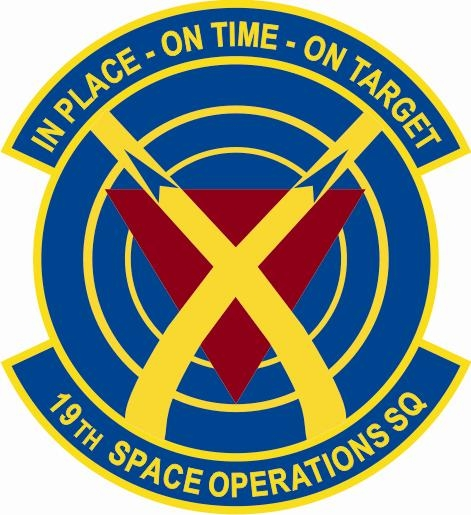
\includegraphics[width=0.6\textwidth]{images/19sops.JPG}
%            \end{figure}
%            U.S. Air Force Reserve's\\
%            19th Space Operations Squadron
%        \end{column}
%    \end{columns}
%    ~\\~\\
%    \centering{\small [gps.gov]}
%\end{frame}

\begin{frame}{Historische Meilensteine}
    \begin{columns}
        \begin{column}{0.5\textwidth}
            \begin{itemize}
                \item[1957:] Sputnik
                \item[1964:] US-Marine, TRANSIT System
                \begin{itemize}
                    \item Bill Guier (Mathematiker)
                    \item George Weiffenbach (Physiker)
                \end{itemize}
                \item Kalter Krieg, Entwicklung verschiedener Systeme
                \item[1973:] Vereinigung zu NAVSTAR
                \item[1974:] Auftrag an Rockwell International
                \item[1986:] Start mit 18 Satelliten
                \item[1995:] 24 Satelliten
                \item[2010:] 30+ Satelliten im Betrieb
            \end{itemize}
        \end{column}
        \begin{column}{0.35\textwidth}
            \begin{figure}
                \centering
                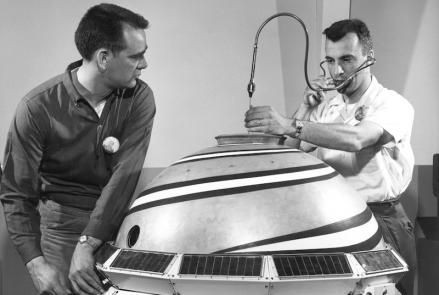
\includegraphics[width=0.35\paperwidth]{images/transit-satellite.jpg}
            \end{figure}
            Tests am zweiten Transit Satelliten, {\small [TimeAndNavigation]}
        \end{column}
    \end{columns}
\end{frame}
